\chapter[Introdução]{Introdução}
\addcontentsline{toc}{chapter}{Introdução}

Este trabalho apresenta a proposta de um projeto de abastecimento de água potável a partir da captação da umidade do ar.
Neste capítulo é apresentada uma descrição do problema, as principais justificativas,
os objetivos e a metodologia de gerenciamento do projeto. 

\section{Contexto}

Água, de todos os recursos naturais, o mais importante, extremamente essencial para a manutenção da vida na Terra.
Não há nenhuma forma de vida que não tenha necessidade de água para sua sobrevivência e desenvolvimento. 

A água doce é também base de atividades econômicas e sociais, como por exemplo, o abastecimento público, agricultura,
pecuária, turismo e está relacionada muita das vezes a matriz energética de um país. 

Denominada cientificamente como “hidróxido de hidrogênio” ou “monóxido de di-hidrogênio, a água é uma substância química
cuja moléculas são formadas por dois átomos de hidrogênio e um de oxigênio. É encontrada em grande quantidade no Universo,
inclusive no planeta Terra, onde cobre parte de sua superfície e é o maior constituinte dos fluídos dos seres vivos. 

O Brasil é o quinto maior país em extensão do mundo com 8.547.403,5 km$^2$,
localizado na parte centro-oriental da América do Sul , ocupa 47,7\%  da área deste continente, cortado pela Linha do Equador
e pelo Trópico de Capricórnio. Possui uma extensa diversidade climática por consequência de vários elementos como a configuração
geográfica, altitudes, relevos, dinâmicas das massas de ar e principalmente pela sua extensão territorial. 
Como consequência o país recebe um abundante índice pluviométrico que varia, sobre mais de 90\% de seu território,
encontrando-se entre 1.000 e mais de 3.000 mm/ano \cite{reboucas03}.

A macrorregião geoeconômica Nordeste (1.1.219.000 km$^2$) é a segunda mais populosa do país (42.822.100 habitantes em 1990). 
Situado entre 	as latitudes 1º e 18º 30’ S e as longitudes 34º 30’ e 40º 20’ W.
A região abrange os estados do Maranhão, Piauí, Ceará, Rio Grande do Norte, Paraíba, Pernambuco, Alagoas, Sergipe e Bahia, nos
quais vivem 18,5 milhões de pessoas e dos quais 8,6 milhões estão na zona rural \cite{cirilo}.

O clima da porção semi-árida é tipificado por um regime de chuvas fortemente concentrado em quatro meses (fevereiro-maio) e
uma grande variabilidade interanual. As extensas secas que fragilizam a região sempre modelaram o comportamento das populações
e foram de grande relevância para a construção de políticas públicas regionais.

O denominado Polígono das Secas, criado pela Lei nº 175 de janeiro de 1936, foi definido por esta, como área a ser objeto das
políticas de combate às secas. O Polígono
abrange oito Estados do Nordeste e um do Sudeste, são eles: Alagoas, Bahia, Ceará, Minas Gerais, Paraíba, Pernambuco, Piauí, Rio Grande do Norte e Sergipe. Composto de diferentes zonas geográficas, com diversos índices de aridez.
Em algumas delas o balanço hídrico é acentuadamente negativo, onde somente se desenvolve a caatinga hiperxerófila sobre solos
delgados. Em outras, verifica-se balanço hídrico ligeiramente negativo, desenvolvendo-se a caatinga hipoxerófila. 
Existem também áreas, de balanço hídrico positivo e presença de solos bem desenvolvidos. Contudo, na área delimitada pela 
poligonal, ocorrem, periodicamente, secas anômalas que se traduzem na maioria das vezes em grandes calamidades, ocasionando 
sérios danos à agropecuária nordestina e graves problemas sociais.

O Estado do Rio Grande do Norte possui área territorial de 52,7 mil de km$^2$ sendo o 22º estado brasileiro em dimensões 
territoriais, correspondente a 0,62\% do tamanho do Brasil, e 3,4\% da região nordeste. 
Limita-se ao norte e a leste com o Oceano Atlântico, ao sul com o Estado da Paraíba e a oeste com o Estado do Ceará.

O Estado historicamente sofreu desastres naturais intimamente conectados à estiagem e à seca. 
As estiagens, quando comparadas às secas, são menos acentuadas e caracterizam-se pela menor intensidade e por menores
períodos de tempo. Já a seca, é caracterizada por longos períodos sem chuva e consequências severas para a região. 
A seca atinge dezenas de municípios do Rio Grande do Norte, dizimando animais e ameaçando de forma por vezes consistente 
a sobrevivência de milhares de famílias, é consideravelmente o problema mais grave que vem afetando a região.

Dentro de toda essa região descrita anteriormente se encontra o município de Acari, situado mais especificamente na 
região do Seridó, na Mesorregião Central Potiguar, no estado do Rio Grande do Norte, no Brasil. De acordo com uma estimativa
realizada pelo IBGE (Instituto Brasileiro de Geografia e Estatística) no ano 2014, sua população é de 11.349 habitantes, e
com uma área de 610,3 quilômetros quadrados.

A seca na região compromete os reservatórios de água resultando em sede, fome e na perda de rebanho, bem como em problemas
de risco à vida humana. Também é atingida, negativamente, a dinâmica ambiental e a conservação do ambiente, pois a falta de 
chuva proporciona o risco de queimadas de forma mais elevada.

Têm-se caracterizado assim o problema a ser reivindicado neste projeto: a ocorrência de secas no território brasileiro,
suas consequências, o discurso de políticos pedindo intervenções políticas de cunho nacional e o uso de medidas técnico 
científicas por parte de instituições públicas no intuito de dar segurança a produção e a sociedade sertaneja, principalmente 
no estado do Rio Grande do Norte e mais especificadamente no município de Acari.


\section{Justificativa}

O diagrama de \textit{Fishbone} que mostra as causas do problema levantado se encontra em anexo no final do arquivo.

\textbf{Por que deve-se pensar em projetos como esse?}

Atualmente, cerca de 40\% da população mundial sofre com consequências da falta de água, além da sede faltam recursos hídricos,
o que gera graves implicações na economia e política. De acordo com o geólogo Sjiklomanov, do Instituto Hidrológico Estadual 
de São Petesburgo, Rússia, em 2000 foi previsto que: “Os países em desenvolvimento vão aumentar seu uso de água em até 200\% em
25 anos”. Em 2014 no Brasil, foi evidenciado consequências desse aumento no consumo de água juntamente com fatores climático,
resultando na falta de água em cidades de Pernambuco, Minas Gerais e São Paulo.

Essa situação de falta de água não é nova, a ONU em 2003 já previa os futuros transtornos que seriam causados pela crise de 
água. O World Water Development Report, se destaca sobre o tema porque é um documento da ONU que também traz estudos mostrando
como esse problema já afeta e mata milhares de pessoas. Este estudo prevê que 2,7 bilhões de seres humanos – 45\% da população 
mundial – vão ficar sem água no ano 2025.

Diante dessa situação e de previsões sobre a falta de água tão breves, devem-se tomar medidas para minimizar a situação e
planejar soluções para a produção de água potável buscando outras fontes, como o ar, por exemplo. Por isso, esse projeto visa
através da umidade do ar, retirar água potável e planeja um estudo de abastecimento na cidade de Acari, RN.

\textbf{Por que  Acari foi a cidade escolhida?}

Na situação de crise hídrica vivida pelo país atualmente, observa-se grandes centros urbanos sofrendo com a falta de água
para consumo humano (o que antes era praticamente exclusivo para a região do semiárido nordestino). Além disso, observa-se que
a seca na região nordeste vem se agravando muito nos últimos anos, especificamente na região do Seridó, que fica no semiárido do RN.

Dessa forma, soluções alternativas para o abastecimento de água potável a fim de atender o consumo humano fazem-se necessárias. 
Sendo assim, a região para a qual o sistema será projetado será o município de Acari – RN, pois é uma região onde há muita
demanda (11303 habitantes) e tem sofrido muito com a escassez de água. A escolha dessa região baseia-se principalmente na 
questão social, uma vez que o projeto visa atender o consumo humano de pessoas que não tem acesso à água potável.

Além de ser uma região que apresenta necessidade de um planejamento para a amenização ou suprimento da escassez de água, é 
também, uma região muito quente, com temperatura média anual de 33Cº, pois está localizada no polígono das Secas 
(local de maior concentração de seca no país). Consequentemente, o volume de água do Açude de Gargalheiras, açude este que
abastece a cidade, decai consideravelmente em épocas de seca, fazendo com que haja escassez de água na cidade. A possibilidade
de retirar água potável do subterrâneo, é inviável pois a água é muito salobra. Apesar de clima quente e semi-árido a umidade
do ar nessa região  possui uma média anual de 60\%, o que possibilita a implantação de tecnologias que aproveitam a umidade do ar
para transformar em água potável.

\textbf{Por que se escolheu o bairro Vereador Tarcísio Bezerra Galvão?}

De acordo com o censo 2010 o bairro Vereador Tarcísio Bezerra Galvão tem cerca de 900 habitantes onde a maioria, cerca de 60\%,
possui entre 15 e 64 anos. Sua localização foi uma das principais motivações para a escolha do bairro, pois é um bairro muito
próximo do Açude de Gargalheiras, e uma das áreas a ser planejada nesse projeto é em relação à distribuição da água, ou seja,
o açude pode facilitar essa distribuição.

\section{Escopo do projeto}

  O projeto consiste em elaborar o projeto de uma planta de abastecimento captação de água a partir da umidade do ar, para amenizar
  o impacto da falta de água potável na região. Para o correto funcionamento da planta de abastecimento, a mesma conta com um sistema
  de monitoramento de qualidade da água, um sistema de gestão da informação e uma matriz energética própria.

  O local da implantação será a cidade de Acari (município da Microrregião do Seridó Oriental, na região do Seridó), no Rio Grande 
  do Norte, no bairro Vereador Tarcísio Bezerra Galvão. Além de atender os requisitos de facilidade de locomoção até a instalação,
  proximidade ao ponto de consumo da energia, espaço necessário para manutenções, não é uma área muito fria, não tem prédios, árvores,
  plantações e construções elevadas (diminuem a velocidade do vento e causam turbulência). Ainda há o fato do bairro sofrer 
  constantemente com a falta de água, pois o açude Gargalheiras, que abastece os municípios de Acarí e Currais Novos, atingiu o 
  pior volume de água de toda a sua história. O reservatório, que tem capacidade de aproximadamente 44 milhões de metros cúbicos
  de água, está com pouco mais de 8\% do total, deixando diversas pessoas em má situação. O bairro tem uma população de 
  aproximadamente 900 habitantes.

  Segundo a Organização Mundial da Saúde (OMS), a quantidade média de água necessária para uma pessoa é de 20L por dia, incluindo
  a água para o preparo de alimentos e higiene pessoal. O projeto visa atender a 25\% dessa quantidade para os 900 habitantes
  do bairro escolhido. Para tal, será necessário o uso de 5 aerogeradores, o que acarreta numa produção média de 5000L, uma vez
  que cada aerogerador gera em média 1000L de água.
  
  \subsection{Localização da implantação do sistema de captação de água}
  
    O sistema de captação de água será localizado nas proximidades do reservatório Gargalheiras, mais precisamente na encosta
    noroeste do açude. Tal localização é justificada pelo padrão do vento na região, padrão hidrográfico da região, padrão
    topográfico da região e área efetiva da encosta e área efetiva do topo parcialmente plano da encosta.
    
    Segundo o INPE, a região apresenta um padrão de ventos na maioria das vezes provenientes da direção sudeste (SE), leste-sudeste
    (ESE) e Leste (E), o qual atinge uma velocidade média de no mínimo 15 km/h.
    
    \begin{figure}[h]
    \begin{center}
      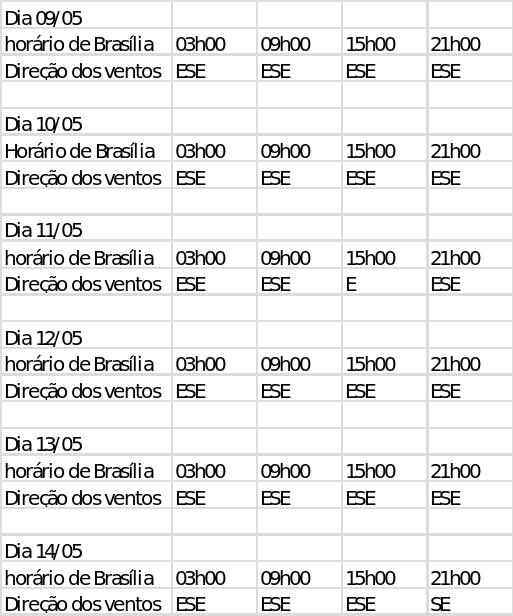
\includegraphics[scale=0.6]{editaveis/figuras/estudo_ventos}
      \caption[Direção dos ventos na região]{Direção dos ventos na região. \footnotemark}
      \label{estudo_ventos}
    \end{center}
    \end{figure}
    \footnotetext{Fonte: Instituto de Pesquisas Espaciais (INPE). Disponível em <http://www.cptec.inpe.br/cidades/tempo/268>.}
    \FloatBarrier
    
    \begin{figure}[h]
    \begin{center}
      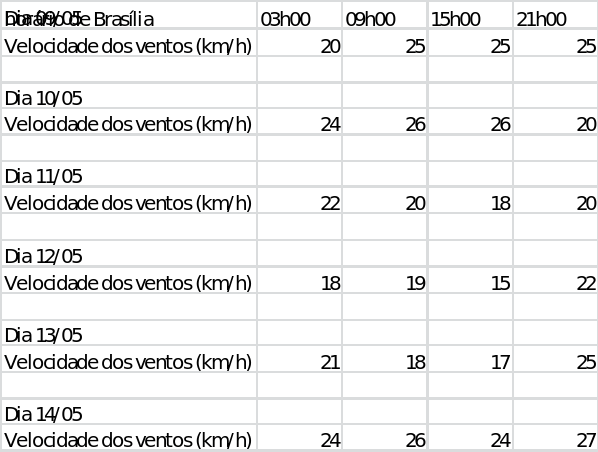
\includegraphics[scale=0.6]{editaveis/figuras/velocidade_ventos}
      \caption[Velocidade dos ventos na região]{Velocidade dos ventos na região. \footnotemark}
      \label{velocidade_ventos}
    \end{center}
    \end{figure}
    \footnotetext{Fonte: Instituto de Pesquisas Espaciais (INPE). Disponível em <http://www.cptec.inpe.br/cidades/tempo/268>.}
    \FloatBarrier
    
    O reservatório Gargalheiras se localiza entre duas encostas, uma posicionada a noroeste e outra a sudeste, o foco das
    operações de implantação do projeto é a encosta posicionada a noroeste, devido aos padrões de ventos na região virem da 
    direção opostos a essa encosta.
    
    \begin{figure}[h]
    \begin{center}
      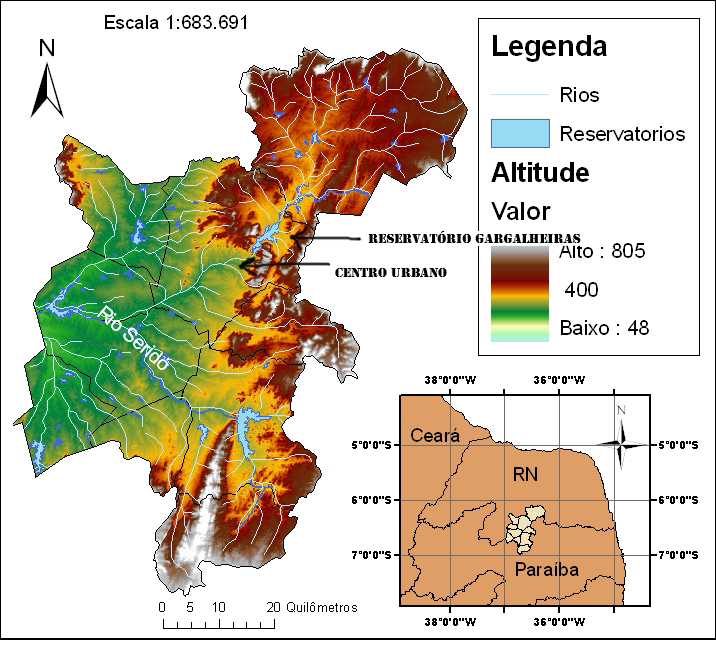
\includegraphics[scale=0.4]{editaveis/figuras/mapa_topografico}
      \caption[Mapa hidrográfico e topográfico da região]{Mapa hidrográfico e topográfico da região. Fonte: \cite{olimpio07}}
      \label{mapa_topografico}
    \end{center}
    \end{figure}
    \FloatBarrier
    
    A área total de disponível nessa encosta, considerando toda a área ingrime lateral e o topo parcialmente
    plano são de 7,71 km $^2$, como ilustram as figuras ~\ref{mapa_area_1} e ~\ref{mapa_area_1_dados}.
    
    \begin{figure}[h]
    \begin{center}
      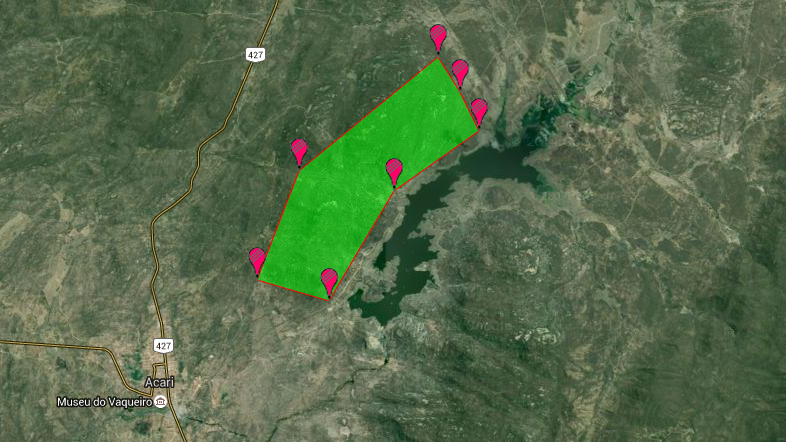
\includegraphics[scale=0.6]{editaveis/figuras/mapa_area_1}
      \caption[Mapa da área total da região de implantação]{Mapa da área total da região de implantação. \footnotemark}
      \label{mapa_area_1}
    \end{center}
    \end{figure}
    \footnotetext{Fonte: http://www.daftlogic.com/}
    \FloatBarrier
    
    \begin{figure}[h]
    \begin{center}
      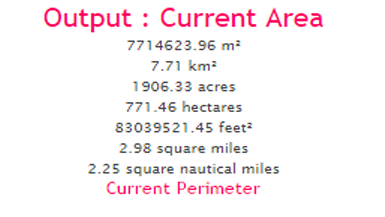
\includegraphics[scale=0.6]{editaveis/figuras/mapa_area_1_dados}
      \caption[Dados sobre a área de implantação]{Dados sobre a área de implantação. \footnotemark}
      \label{mapa_area_1_dados}
    \end{center}
    \end{figure}
    \footnotetext{Fonte: http://www.daftlogic.com/}
    \FloatBarrier
    
    Analisando só o topo, que se apresenta razoavelmente plano na encosta, a área disponível para implementação do projeto será de
    3,86 km$^2$ e sua distância efetiva será de 6,383 km, distância que vai da cabeceira sudoeste do reservatório à cabeceira nordeste
    do mesmo, como ilustram as figuras ~\ref{mapa_area_2} e ~\ref{mapa_area_2_dados}.
    
    \begin{figure}[h]
    \begin{center}
      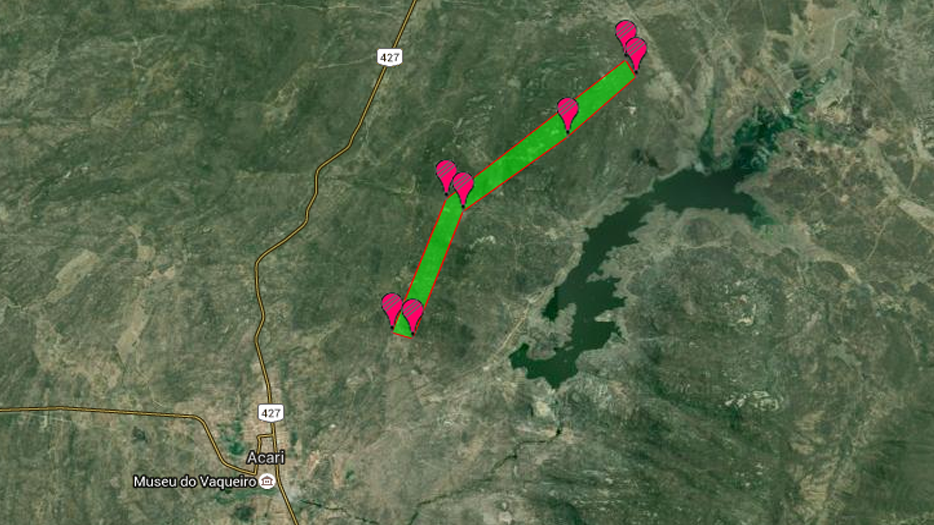
\includegraphics[scale=0.5]{editaveis/figuras/mapa_area_2}
      \caption[Mapa da área do topo da região de implantação]{Mapa da área do topo região de implantação. \footnotemark}
      \label{mapa_area_2}
    \end{center}
    \end{figure}
    \footnotetext{Fonte: http://www.daftlogic.com/}
    \FloatBarrier
    
    \begin{figure}[h]
    \begin{center}
      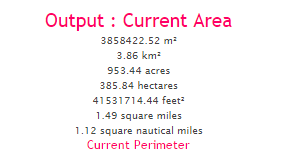
\includegraphics[scale=0.8]{editaveis/figuras/mapa_area_2_dados}
      \caption[Dados sobre a área do topo]{Dados sobre a área do topo. \footnotemark}
      \label{mapa_area_2_dados}
    \end{center}
    \end{figure}
    \footnotetext{Fonte: http://www.daftlogic.com/}
    \FloatBarrier
   
   \subsection{Distribuição da água}
   
    A distribuição da água será realizada através de torneiras acopladas a parte externa da torre de controle, com acesso direto ao produto final. O local o qual se implantará esse sistema será em uma praça no bairro vereador Tarcísio Bezerra Galvão na cidade de Acari.
    
    Como um dos requisitos é criar um local priorizando o social e a conscientização por parte da população, logo, a praça deverá ser um espaço público de enfoque educativo. Ela necessita possuir informes sobre sustentabilidade, conservação da natureza e uso consciente de todos os recursos naturais, principalmente da água, que será o objetivo de todo o projeto.
    
    No entanto, a construção e manutenção dessa praça é de inteira responsabilidade da empresa e/ou Prefeitura Municipal de Acari que irá implementar e se utilizar da tecnologia desenvolvida pela PA31, Planta de Abastecimento de Água Através do Ar. A empresa PA31 fornecerá somente o básico de um local de distribuição o qual conteria as torneiras, torre de controle, local para cadastro de pessoas, além da tecnologia de interesse, portanto, não se responsabilizando pelo design e despesas relativas a essa praça.
      
    O local para cadastro de pessoas ficaria ao lado do local de distribuição realizada pelas torneiras públicas e da distribuição das garrafas contendo o excedente de água produzido pelo sistema. Essas garrafas teriam a capacidade variando em 2 a 20 litros, dependendo da garrafa, para poder atender famílias com número variado de membros sendo-as distribuídas de forma gratuita. 
    
    O cadastro de usuários do Bairro Vereador Tarcísio Bezerra Galvão da cidade de Acari – RN possui a finalidade de obter um controle sobre quantas pessoas o projeto está atendendo, qual a população que está utilizando o serviço, qual a população do Bairro, qual a real demanda de água por pessoa. Este controle ajudará a estimar aproximadamente a quantidade de galões de água que serão destinadas ao projeto, além de efetuar um censo interno para que o processo seja melhorado no futuro, atendendo tanto a população local quanto a flutuante. 
    
    Este cadastro será feito de maneira bem simples, em uma planilha eletrônica e a mesma poderá ser modificada diariamente, de acordo com o cadastro de um novo cidadão. Abaixo se encontra um modelo de cadastro de cidadãos do Bairro que pode ser utilizado no projeto:
    
    \begin{figure}[!htbp]
      \centering
      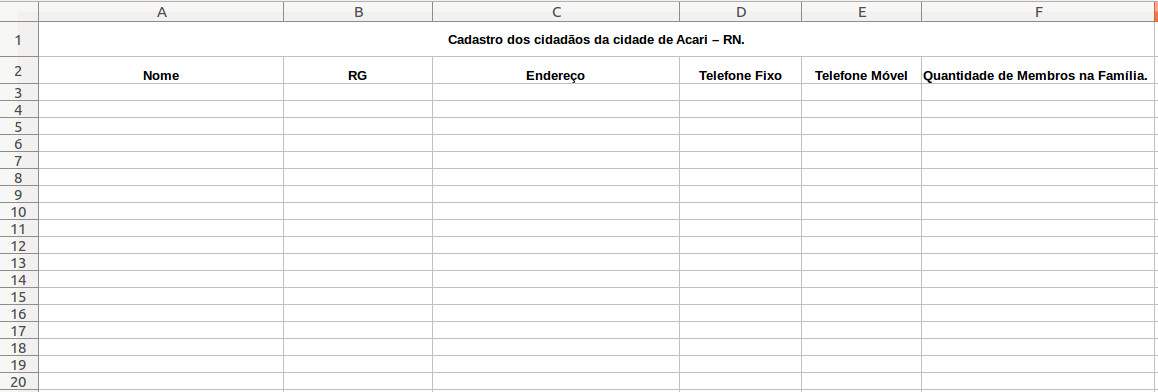
\includegraphics[scale=0.35]{editaveis/figuras/modelo_planilha_controle}
      \caption[Modelo de planilha de controle]
      {Modelo de planilha de controle.}
      \label{modelo_planilha_controle}
    \end{figure}
    
    A água produzida que não atender aos parâmetros previamente estipulados de qualidade para consumo humano, poderá ser introduzida ao sistema de distribuição de água da cidade, para que seja levada a Central de Tratamento do Município de Acari, para que possa ser tratada adequadamente.
    
    A parceria com outras empresas e/ou o Governo do Município de Acari se faz necessário para poder minimizar os custos, aumentar a visibilidade do projeto e das empresas e/ou governos que o ajudaram a implementar, e consequentemente, poder se investir de maneira adequada em projetos sociais. Nos tópicos subsequentes desse texto há a listagem de três possíveis parceiros que poderiam apoiar a implementação de projeto: a Coca-Cola Brasil, Água Mineral Indaiá e a Cristalina de Natal.
    
    Outras justificativas para a escolha dessas empresas são que elas poderiam ceder recipientes (garrafas) que já possuem características higiênicas adequadas, por já trabalharem no ramo e terem controle sobre isso. Além de poderem fazer o descarte futuro dos recipientes de forma adequada, já que cuidam disso atualmente em suas empresas devido à preocupação ambiental que todas possuem.
    
    Essa parceria possibilitaria, também, a distribuição gratuita das garrafas, pois ao invés de cobrarem pela ela, eles ganhariam visibilidade associando sua marca a um projeto inovador, social e ambiental. Essa associação poderia ser evidenciada e comprovada imprimindo o logotipo de empresa que desenvolveu a tecnologia, PA31, e dos implementadores e/ou parceiros.
    
    \subsubsection{Justificativa da escolha do tipo de distibuição}
    
      Este tipo de distribuição foi escolhida por apresentar vários critérios favoráveis de implementação, os quais serão citados abaixo:
      
      \begin{itemize}
       \item Torna a solução socialmente viável, ou seja, a população vai em busca do produto por si mesma, não precisando pagar pelo produto;
       \item O local se tornará um ponto de encontro da sociedade, pois se concentrará em uma praça de intuito educativo;
       \item Geração de visibilidade para toda a cidade;
       \item Estruturalmente mais econômico;
       \item Este tipo de implementação já ocorre em outros projetos;
       \item Capacidade de parcerias públicas e com empresas que tem interesse social.
      \end{itemize}

	Como exemplo de cidade que já adotou esse tipo de distribuição de água temos Roma na Itália com as estruturas de “Nasoni” (nariz em italiano), ou também conhecidas como “fontana” (bebedouro/fonte em italiano). O primeiro nome faz alusão ao formato desses locais de distribuição de água que possuem um grande bico, como pode ser visto nas figuras abaixo, com suas devidas dimensões em centímetros\cite{rodrigues}. 
	
	\begin{figure}[!htbp]
      \centering
      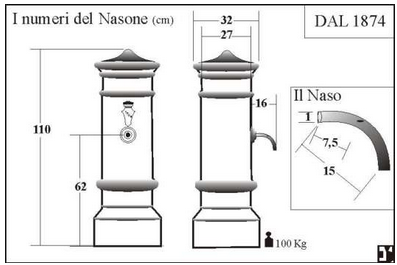
\includegraphics[scale=1]{editaveis/figuras/nasone}
      \caption[Dimensionamento de uma Nasoni]
      {Dimensionamento de uma Nasoni \cite{rodrigues}}
      \label{dimensionamento_nasoni}
    \end{figure}
    
    Essas fontes foram resultado de uma iniciativa do funcionário municipal Rinazzi, em 1874. Há registros que comprovam a implantação de mais de 2500 dessas fontes, que saem água potável durante todo o dia \cite{abc}. A iniciativa deu tão certo que desde 1990 toda a população rural da Itália (100\%) tem acesso à fonte de água potável enquanto que nessa época, 1990, apenas 61,80\% do mundo tinha esse acesso\cite{bank}.
    
    Portanto esse mecanismo que escolhemos de distribuição é confiável e já resultou em melhorias significativas em outro país. Além de se tornar um ponto turístico na cidade de Acari, RN, como o Nisoni é na Itália, ele poderá melhorar a qualidade de vida das pessoas dessa cidade. Ainda, o mecanismo de abastecimento da PA31 possui vantagens sobre o italiano, pois ele não terá perda de água envolvida quando a população não estiver usando, já que não sairá água de forma livre durante todo o dia como o outro mecanismo, e sim apenas quando abrirem as torneiras. Outras vantagens sobre o Nasoni, é que mecanismo de captação da PA31 , possui um grande aparato tecnológico, é autossustentável, capta a água por meio da umidade do ar, têm vários sensores para averiguar a qualidade da água e ainda poderá fazer um censo interno para averiguar a demanda populacional por água, permitindo então, o melhoramento do sistema com o passar dos anos.
    \FloatBarrier
	\begin{figure}[!htbp]
      \centering
      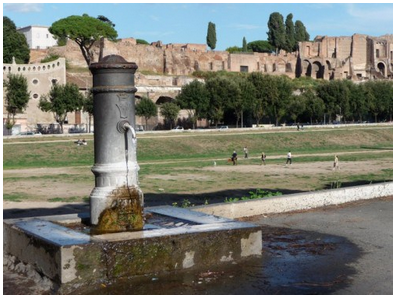
\includegraphics[scale=1]{editaveis/figuras/nasoni_italia}
      \caption[Um Nasoni com o Circo Massimo e o Palatino ao fundo em Roma, Itália ]
      {Um Nasoni com o Circo Massimo e o Palatino ao fundo em Roma, Itália  \cite{rodrigues}}
      \label{dimensionamento_nasoni}
    \end{figure}
    \FloatBarrier
    \subsubsection{Possíveis empresas parceiras}
      
      Com a finalidade aumentar a viabilidade listamos três empresas abaixo as quais poderão se tornar parceiras nesse projeto, e que possuem preocupação ambiental e social.
      
      A Coca-Cola Brasil seria uma dessas parceiras, ela é responsável por mais de 125 produtos relacionados com bebidas não 
      alcoólicas, dentre esses produtos cerca de 60\% possuem pouca caloria. Contendo, portanto, experiência no mercado, qualidade 
      já averiguada, em projetos que têm preocupação social, e pedagógica e ambiental. Em uma de suas marcas, Crystal Eco, há
      a venda de água para consumo, o produto apresenta grande marketing em relação ao lado ecológico, diante disso e de várias
      outras campanhas que a Coca-Cola faz referente à sustentabilidade, além de se preocupar com a quantidade de sódio presente
      na água mineral (saúde do consumidor), tornando nosso projeto mais interessante para a mesma. O projeto tem todo potencial 
      para ser utilizada por essa grande empresa \footnotemark.
      \footnotetext{Fonte: <https://www.cocacolabrasil.com.br/nossas-marcas/>.}
      
      
      \begin{figure}[!htbp]
	\centering
	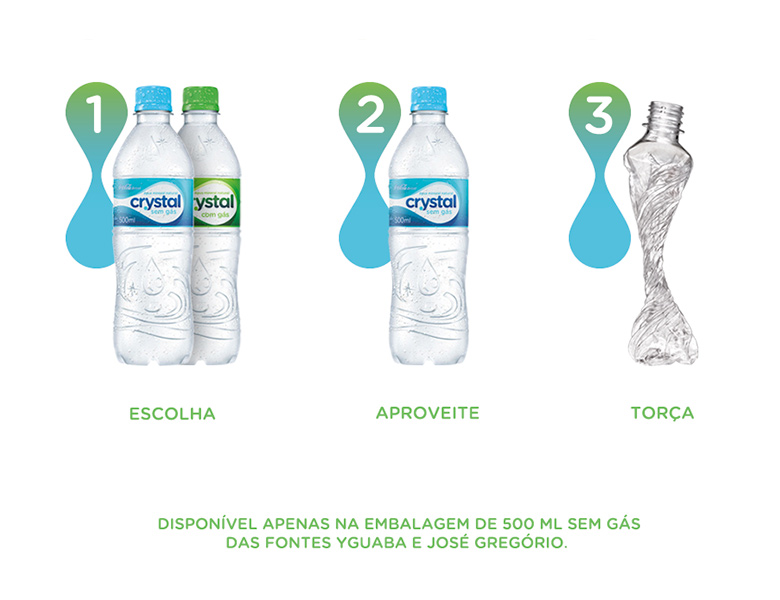
\includegraphics[scale=0.35]{editaveis/figuras/descarte_garrafa_agua}
	\caption[Descarte da Garrafa de água mineral Crystal]
	{Descarte da Garrafa de água mineral Crystal \footnotemark.}
	\label{descarte_garrafa_agua}
      \end{figure}
      \footnotetext{Fonte: <http://www.aguamineralcrystal.com.br/pt/crystal-eco/>.}
      
      Essa marca desenvolvida pela Coca-Cola, Crystal Eco, aplica medidas em seus produtos a fim de contribuir com o lado 
      ecológico: reduziu o nível de desperdício ao reduzir 2/3 do seu antigo volume, suas embalagens são 100\% recicláveis,
      e a mais nova embalagem de sua garrafa mineral é fácil de transporte e armazenagem por poder ser torcida reduzindo 37\%
      do seu volume \footnotemark.
      \footnotetext{Fonte: <http://www.aguamineralcrystal.com.br/pt/crystal-eco/>.}
      
      Outra empresa seria a Indaiá, a qual é pertencente ao Grupo Edson Queiroz, a maior indústria de águas minerais do país, 
      abrangendo 40 fontes em mais de 15 estados \footnotemark.
      \footnotetext{Disponível em: <http://www.indaia.com.br/site/>.}
      Ela é a primeira empresa do Brasil da indústria de águas minerais
      a ter todos os seus processos e áreas certificados pela ISO 9001 (normas responsáveis pela eficácia de gestão da empresa e
      qualidade de seus produtos) \cite{iso9001}.
      
      Portanto, a Indaiá por abranger vários estados, dentre eles outros locais propícios à instalação do projeto capaz de retirar 
      água do ar já que a empresa tem grande potencial industrial e características inovadoras. Atualmente, ela tem expandido na
      atuação no segmento de bebidas sendo referência no mercado e conquistando cada vez mais o gosto e a preferência dos
      consumidores. O projeto da PA31, seria um oportunidade deles associarem sua marca cada vez mais com a inovação dessa
      tecnologia \footnotemark.
      \footnotetext{Disponível em: <http://www.indaia.com.br/site/>.}
	A empresa Cristalina de Natal possui vinte anos de experiência na indústria de água mineral, ela seria uma possível empresa parceira por está localizada na cidade de Macaíba, no Rio Grande do Norte, portanto, tendo proximidade com a cidade de Acari e por já distribuir água mineral em todo o estado do RN\footnotemark. A empresa garante a qualidade de sua água possuindo certificação da ISSO 9001, atestado BPF (Boas Práticas de Fabricação), APPCC (Análise de perigos e Pontos Críticos de controle) e vários prêmios de reconhecimento nacional\footnotemark.
	\footnotetext{Disponível em: <http://www.cristalina.com.br/empresa.php>}
	\footnotetext{Disponível em: <http://www.cristalina.com.br/qualidade.php25>}
	Portanto, como já citado, essas empresas poderiam ser possíveis parceiras para a implementação desse projeto, garantindo qualidade na distribuição e contribuindo para a questão social. Suas marcas seriam associadas ao produto e consequentemente seriam reconhecidas por essas boas práticas em relação ao social, meio ambiente, e qualidade de vida.
      
      

    
\pagebreak
\section{Objetivos}

Este trabalho tem por objetivo propor uma solução que consiga suprir parte da demanda da população. Os esforços que serão
realizados ao longo do período de desenvolvimento, no transcorrer de todas as etapas do processo buscam a qualidade e real
eficácia do produto, ou seja, oferecer a demanda de água do bairro Vereador Tarcísio Bezerra Galvão situado em Aracarí-RN, 
água potável de qualidade.

 \subsection{Objetivos específicos}
 
 São objetivos específicos do projeto:
 \begin{itemize}
  \item Elaborar o projeto mecânico estrutural do sistema de captação de água;
  \item Elaborar o projeto estrutural do sistema de transporte da água para a central de armazenamento;
  \item Elaborar o projeto do sistema de monitoramento e controle da qualidade da água captada;
  \item Elaborar o projeto da matriz energética que dará o suporte para os sistemas de captação de água e monitoramento e controle;
 \end{itemize}

 
\section{Metodologia de Gerenciamento}

A metodologia de gerenciamento do projeto utilizada foi o \textit{Scrum}, que é uma metodologia de gerenciamento de projetos ágil.
O \textit{Scrum} divide o trabalho em \textit{sprints}, que são iterações com um tempo definido, e ao final de cada 
\textit{sprint} é feita uma retroscpectiva para avaliar o que foi feito. No início de cada \textit{sprint},
a mesma é planejada. Todo o trabalho que tem ser feito é caracterizado como \textit{product backlog}, e cada \textit{sprint}
consome parte do \textit{product backlog}, até que o produto final seja obtido.

Alguns artefatos do \textit{Project Management Body of Knowledge} (PMBoK) foram buscados para suporte na gerência do projeto.
Foram utilizados os seguintes planos de gerenciamento do PMBoK como documentos auxiliares:

  \begin{itemize}
  \item Plano de Gerenciamento do Projeto;
  \item Plano de Gerenciamento de Escopo;
  \item Plano de Gerenciamento de Recursos Humanos;
  \item Plano de Gerenciamento de Comunicações;
  \item Plano de Gerenciamento de Aquisições;
  \item Plano de Gerenciamento de Tempo;
  \item Plano de Gerenciamento de Qualidade;
  \item Plano de Gerenciamento de Custos;
  \item Plano de Gerenciamento de Riscos.
  \end{itemize}
  
  Os planos de gerenciamento se encontram em anexos, junto com o termo de abertura do projeto e a declaração de escopo.
  
  \subsection{Resumo da Gerência de Projeto}
  
      No primeiro momento de pesquisa para a definição do local e tecnologia da solução e para a elaboração dos planos,
      a equipe de desenvolvimento foi divida em nove grupos seguindo as nove áreas de conhecimento do PMBoK.
      Foi definido um gerente geral para coordenar as atividades iniciais junto a um grupo de suporte a decisão, 
      e também foram definidos responsáveis para cada frente de pesquisa.
      Essa organização primária permitiu um melhor rendimento do grupo para a criação dos planos de gerenciamentos, pois cada
      um trabalhou na área que mais se encaixava no seu perfil, além de possibilitar grupos pequenos para a pesquisa de possíveis
      locais e tecnologias, o que aumentou o alcance das pesquisas.
      
      No momento de execução do planejamento do projeto, que engloba o levantamento do referencial teórico e o resultado das análises
      e projeto da solução, a equipe de desenvolvimento foi separada em quatro times de desenvolvimento e um time de gerência.
      
      Os times de desenvolvimento foram separados conforme a área de atuação dos integrantes para trabalharem cada um em uma frente
      específica de trabalho relacionada com sua área. Cada time de desenvolvimento possuía um líder, denominado de 
      \textit{Scrum Master}, que é responsável por guiar e assistir o time no que fosse necessário durante as \textit{sprints}.
      
      O time de gerência é composto por dois integrantes da equipe.
      Os integrantes do time de gerência, denominados de \textit{Product Manager}, são os responsáveis por gerenciar e acompanhar 
      todos os times de desenvolvimento, realizar validação inicial de documentos e demais textos,
      manter os \textit{backlogs} e o relatório, e executar demais atividades relacionadas à gerência do projeto.
    
    \begin{figure}[!h]
      \centering
      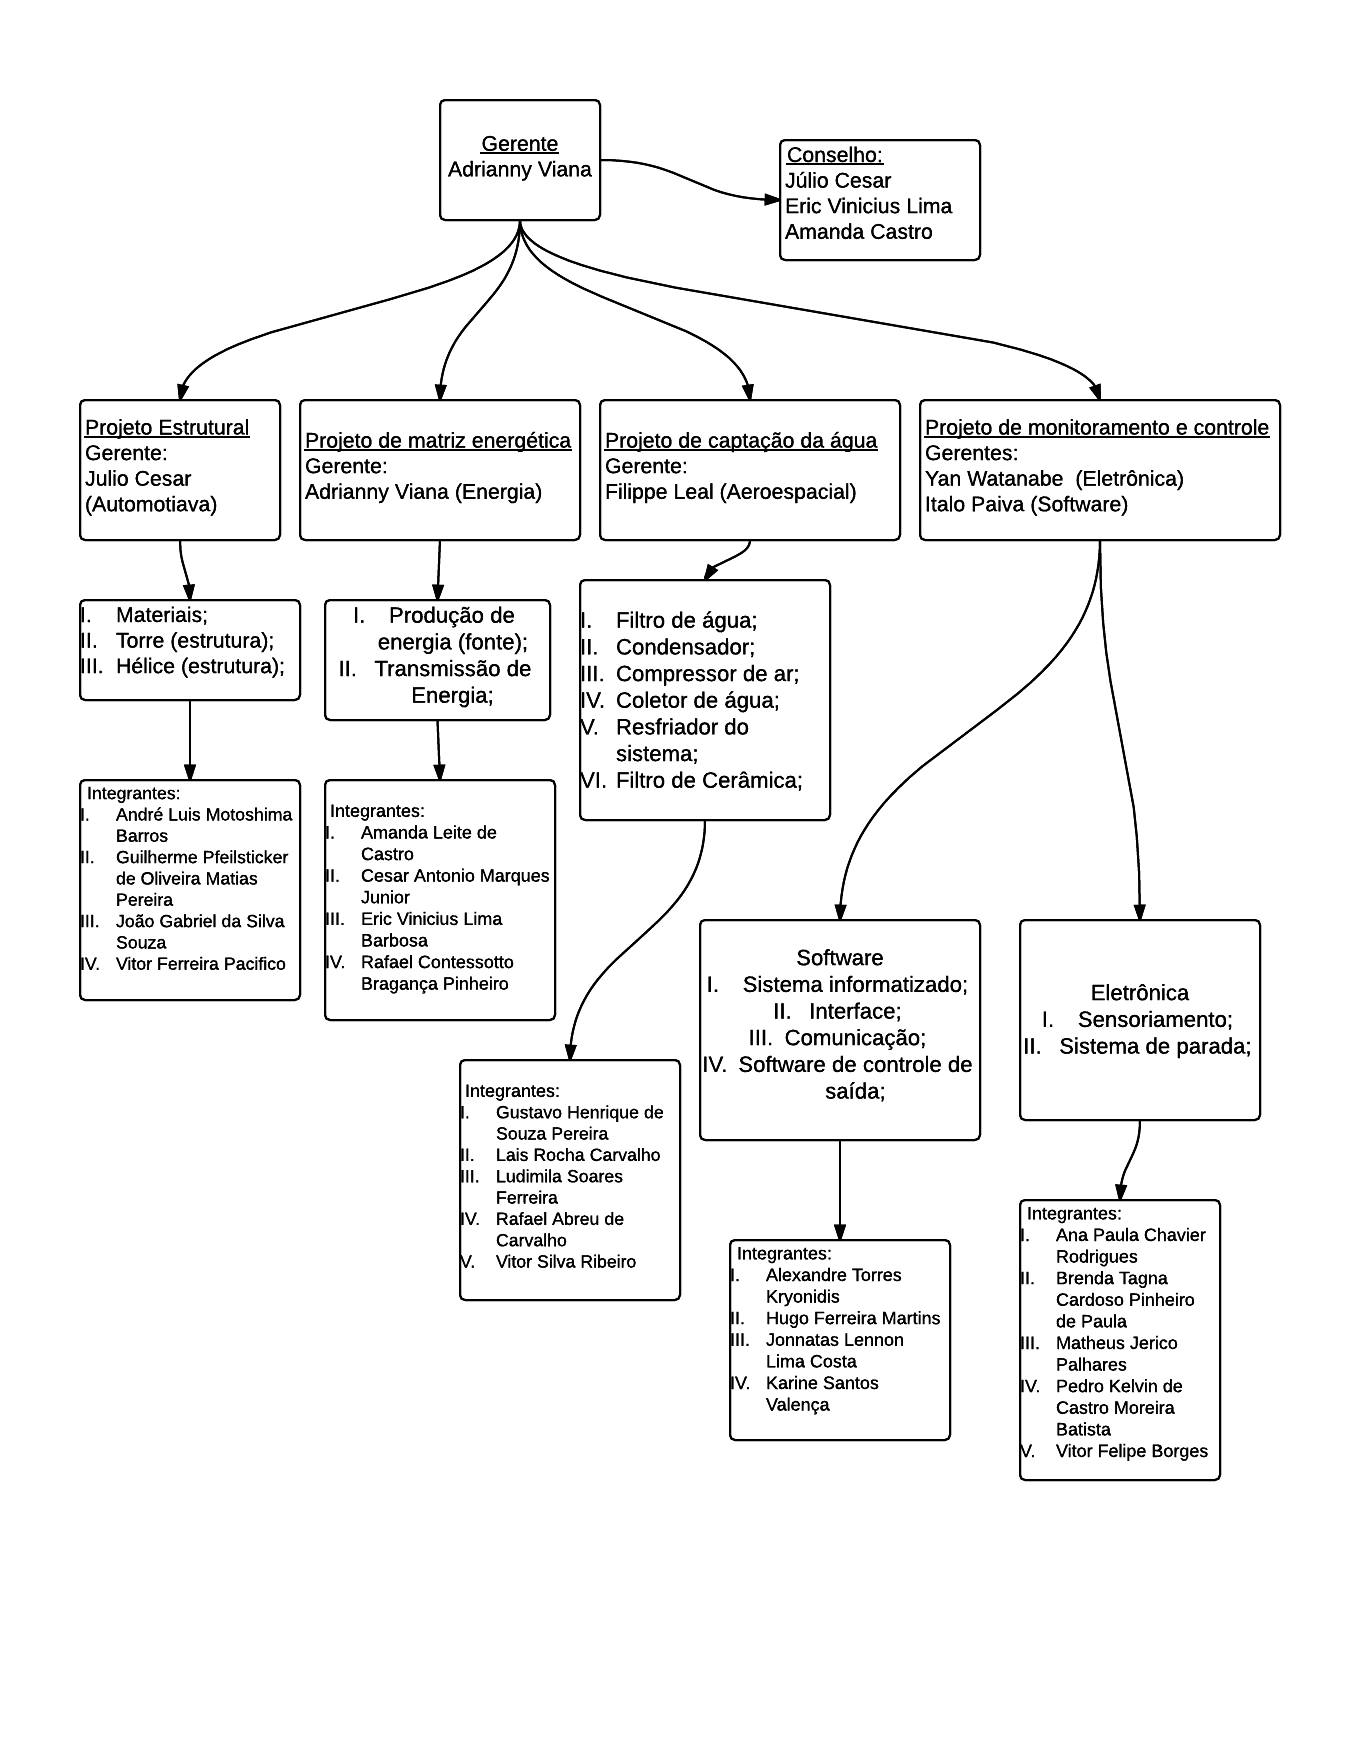
\includegraphics[scale = 0.27]{editaveis/figuras/Fluxograma_gerencia}
      \label{fluxograma_gerencia_projeto}
      \caption{Fluxograma da gerência do projeto}
    \end{figure}
    \FloatBarrier
    
  \pagebreak
  \subsection{Estrutura Analítica do Projeto}
    
    A Estrututura Analítica do Projeto abaixo mostra os entregáveis do projeto ao longo do tempo de execução.
    
   \begin{figure}[!h]
    \centering
    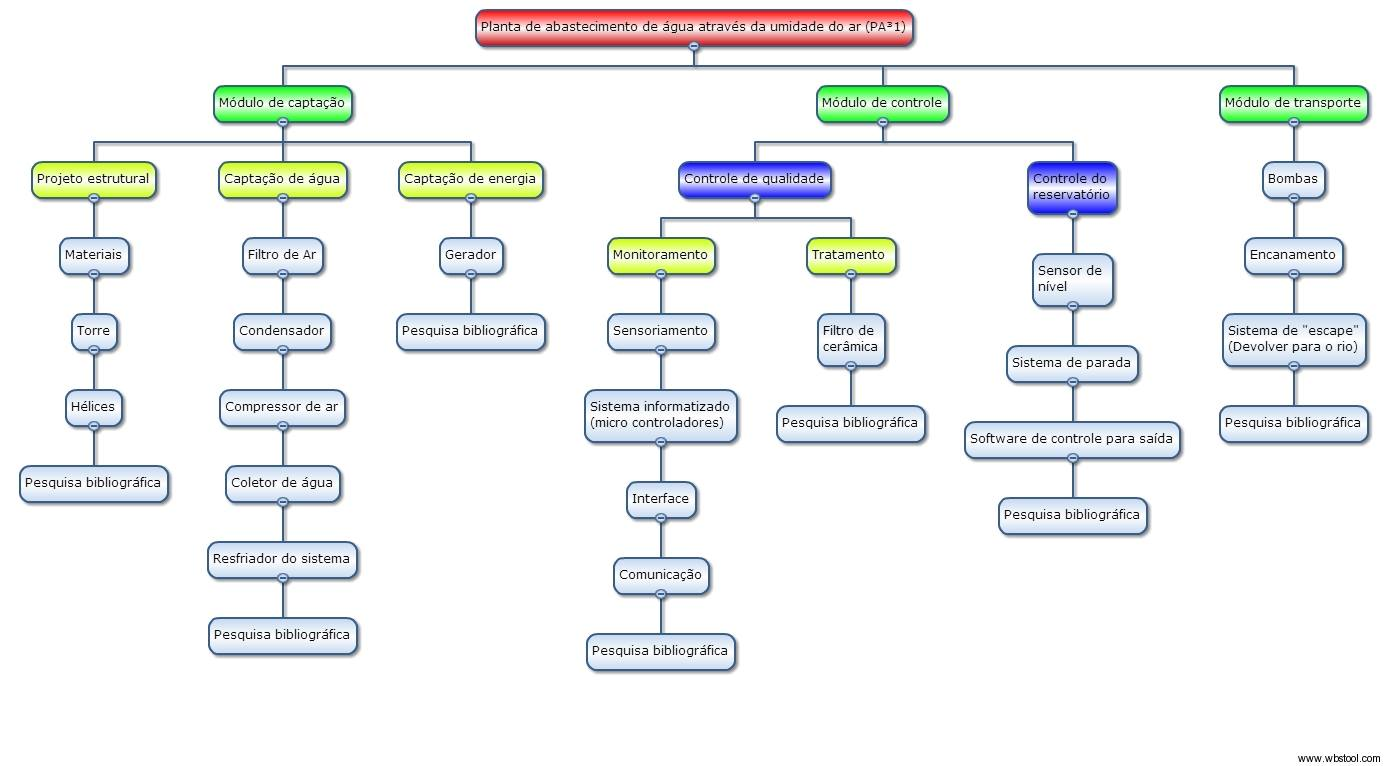
\includegraphics[scale = 0.4, angle=90]{editaveis/figuras/EAP}
    \label{EAP}
    \caption{Estrutura Analítica do Projeto}
   \end{figure}
   \FloatBarrier
   
  \pagebreak
  \subsection{Cronograma}
   
   \textbf{Cronograma de atividades - Ponto de Controle 1}
   \begin{figure}[!h]
    \centering
    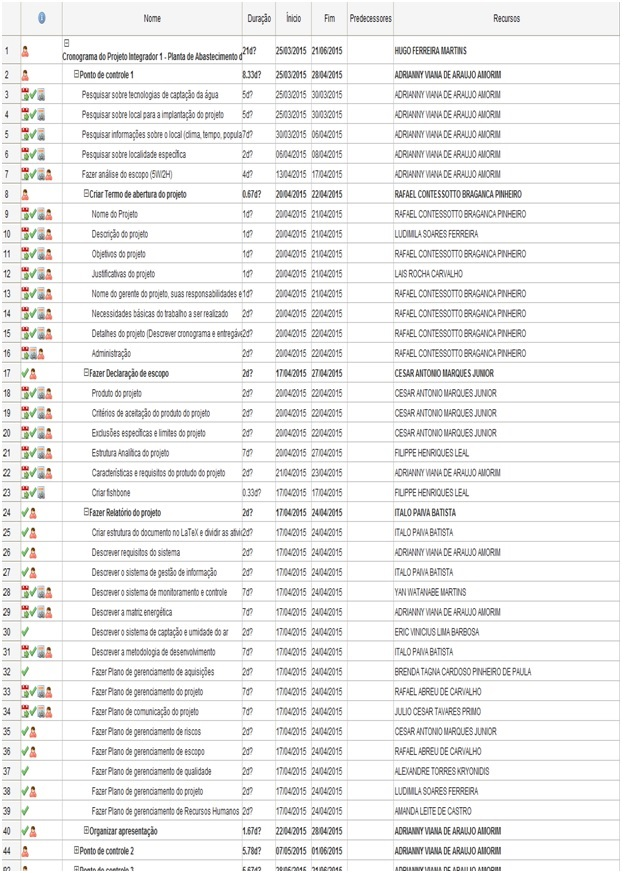
\includegraphics[scale = 0.8]{editaveis/figuras/cronogramaPC1}
    \label{Cronograma de atividades PC1}
    \caption{Cronograma de atividades - Ponto de Controle 1}
   \end{figure}
   \FloatBarrier
   
   \pagebreak
   \textbf{Cronograma de atividades - Ponto de Controle 2}
   \begin{figure}[!h]
    \centering
    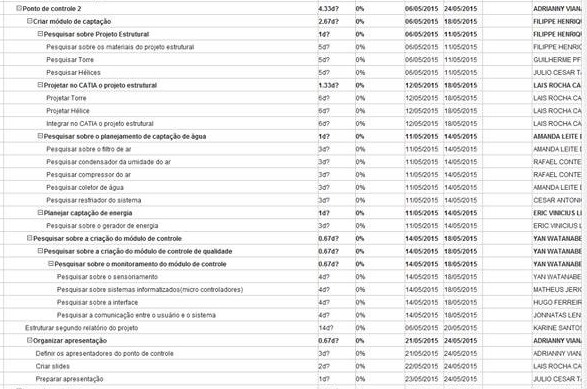
\includegraphics[scale = 0.8]{editaveis/figuras/cronogramaPC2}
    \label{Cronograma de atividades PC2}
    \caption{Cronograma de atividades - Ponto de Controle 2}
   \end{figure}
   \FloatBarrier
   
   \pagebreak
   \textbf{Cronograma de atividades - Ponto de Controle 3}
   \begin{figure}[!h]
    \centering
     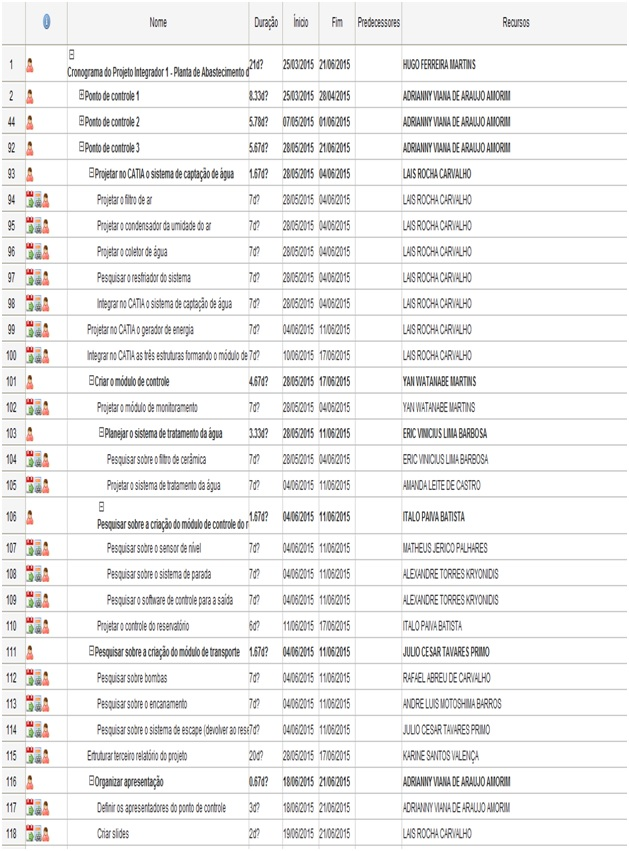
\includegraphics[scale = 0.8]{editaveis/figuras/cronogramaPC3}
    \label{Cronograma de atividades PC3}
    \caption{Cronograma de atividades - Ponto de Controle 3}
   \end{figure}
   \FloatBarrier
   
  \pagebreak
  \textbf{Gráfico de Gantt- Ponto de Controle 1}
   \begin{figure}[!h]
    \centering
    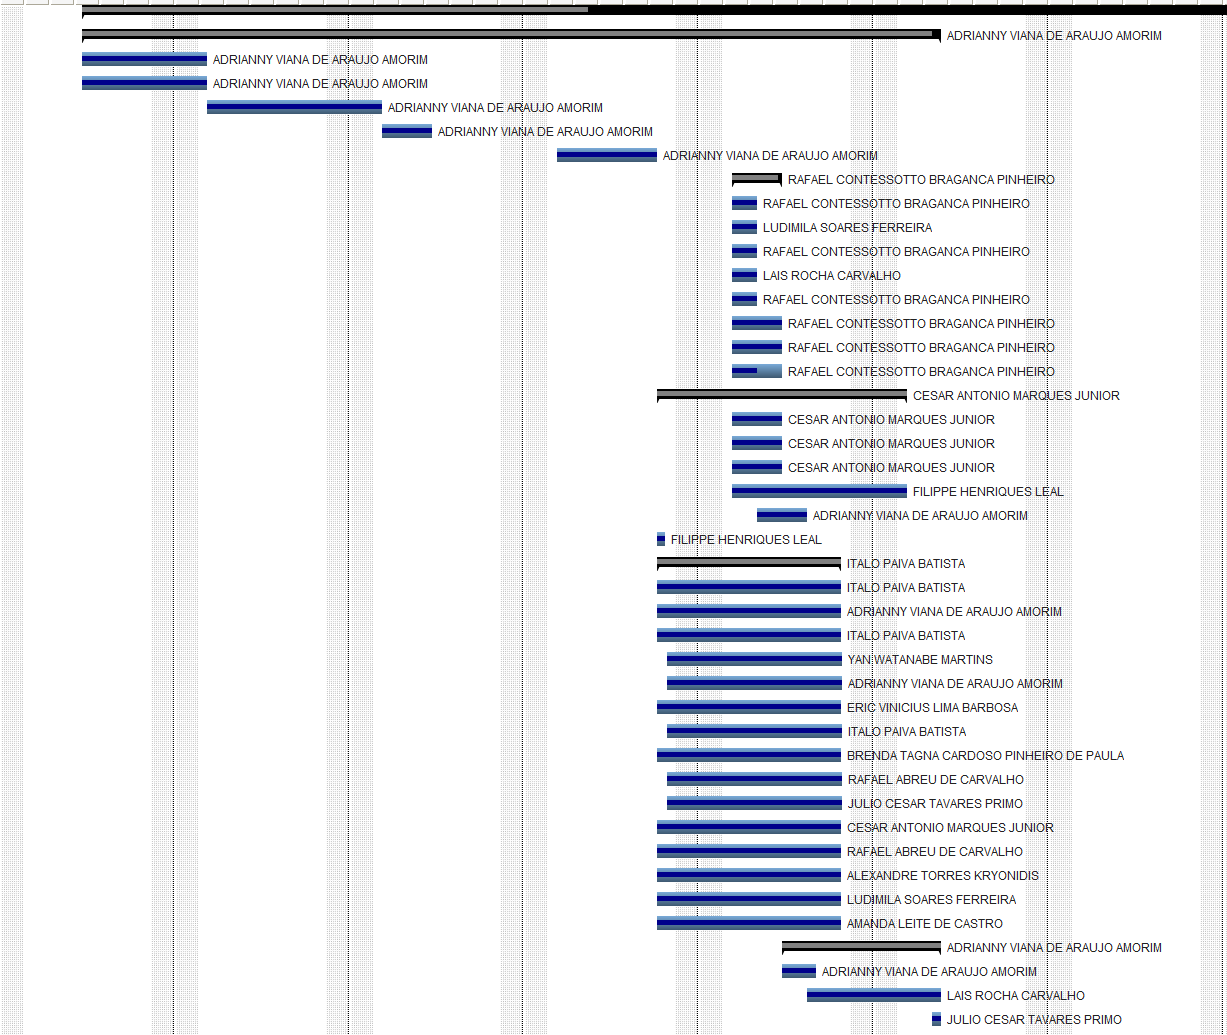
\includegraphics[scale = 0.45]{editaveis/figuras/ganttPC1}
    \label{Gráfico de Gantt PC 1}
    \caption{Gráfico de Gantt - Ponto de Controle 1}
   \end{figure}
   \FloatBarrier
   
  \pagebreak
  \textbf{Gráfico de Gantt- Ponto de Controle 2}
   \begin{figure}[!h]
    \centering
    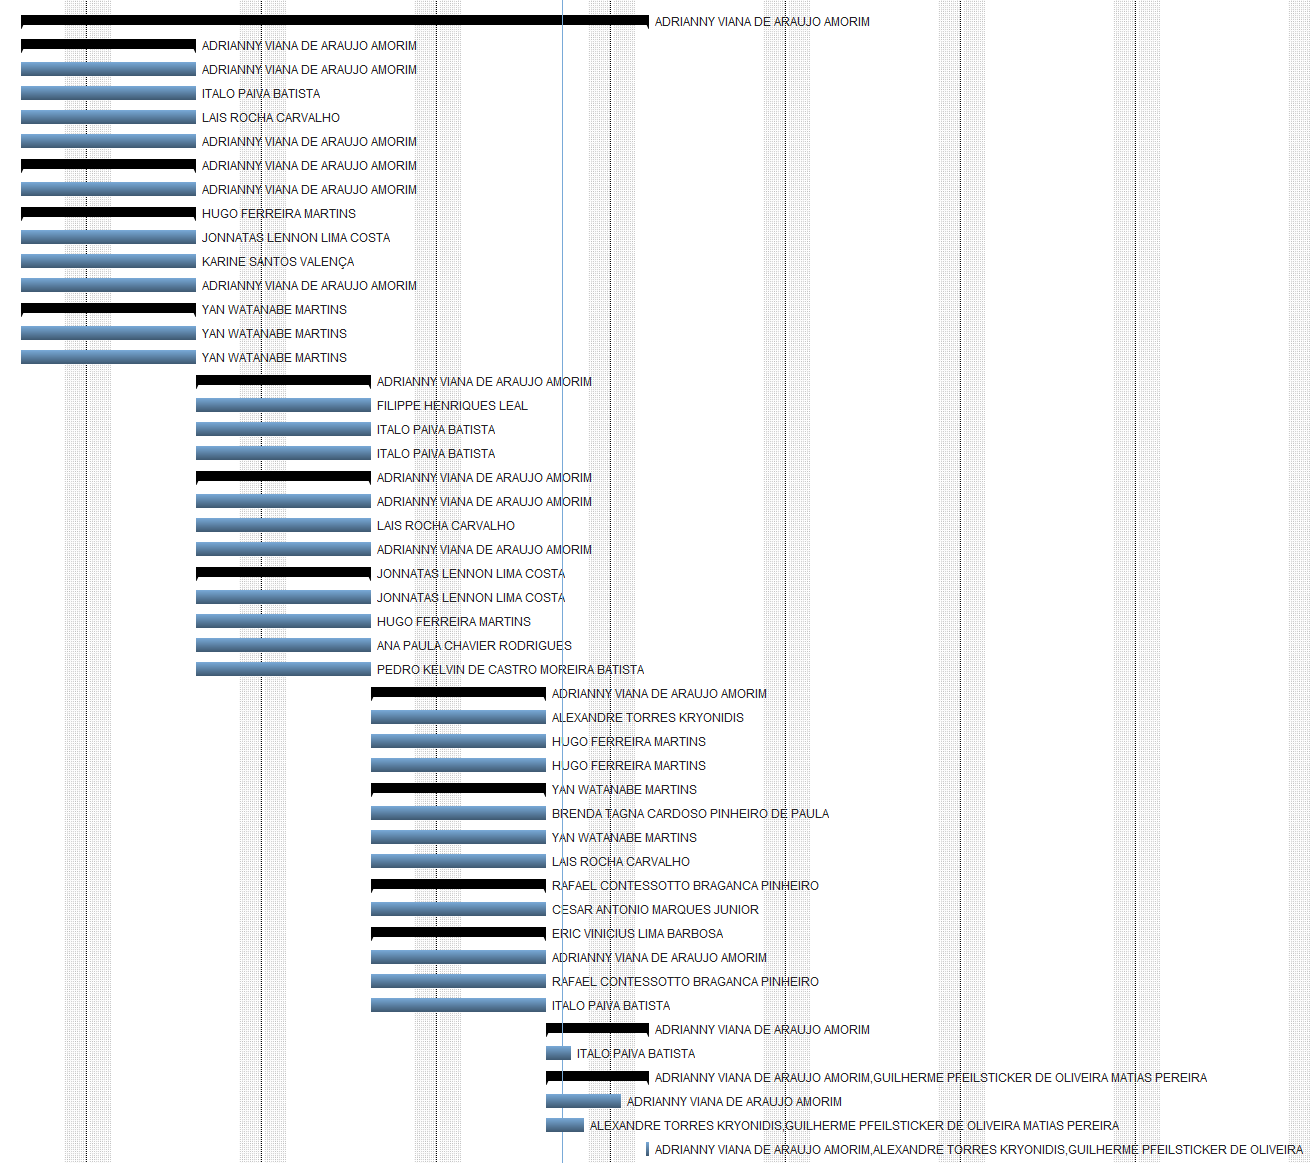
\includegraphics[scale = 0.5]{editaveis/figuras/ganttPC2}
    \label{Gráfico de Gantt PC2}
    \caption{Gráfico de Gantt - Ponto de Controle 2}
   \end{figure}
   \FloatBarrier
   
  \pagebreak
  \textbf{Gráfico de Gantt- Ponto de Controle 3}
   \begin{figure}[!h]
    \centering
    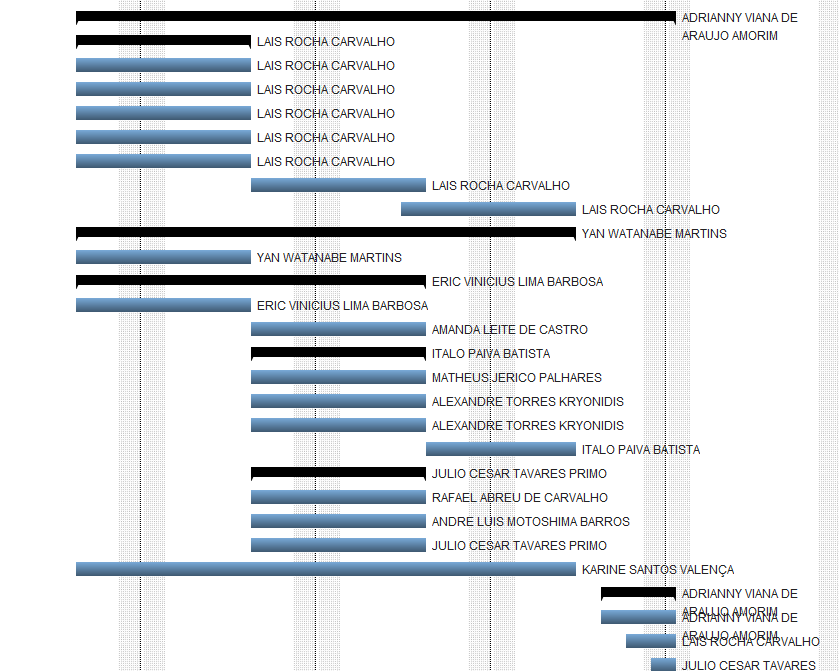
\includegraphics[scale = 0.5]{editaveis/figuras/ganttPC3}
    \label{Gráfico de Gantt PC3}
    \caption{Gráfico de Gantt - Ponto de Controle 3}
   \end{figure}
   \FloatBarrier